\documentclass{article}
\usepackage[utf8]{inputenc}
\usepackage{lmodern}
\usepackage{blindtext}
\usepackage{amsmath}
\usepackage[a4paper, inner=1.7cm, outer=2.7cm, top=3cm, bottom=3cm, bindingoffset=1.2cm]{geometry}
\usepackage{tcolorbox}
\usepackage{graphicx}
\usepackage{wrapfig}
\usepackage{makecell}
\usepackage{boldline}
\usepackage{float}
\usepackage{tabularx}
\usepackage[table]{colortbl}
\usepackage[english]{babel}
\usepackage{amsthm}
\usepackage{hyperref}

\newtheorem*{invariant}{Invariant}

\renewcommand\theadalign{bc}
\renewcommand\theadfont{\bfseries}
\renewcommand\theadgape{\Gape[4pt]}
\renewcommand\cellgape{\Gape[4pt]}

\begin{document}

\title{\textbf{ChickenBonds: Self-Bootstrapping Treasury}}
\author{Liquity Team}
\date{April 12, 2021}

\maketitle

\section*{Abstract}
ChickenBonds is an autonomous self-bootstrapping treasury system that acquires yield-bearing tokens (TKN) through a novel bonding mechanism: users may bond TKN and start accruing a "boosted" derivative token (bTKN) in return.

At any time, bond holders can either retrieve their principal foregoing the accrued amount ("chicken out") or trade it in against the accrued bTKN ("chicken in").

The TKN acquired by the system backs the bTKN supply: while a portion of the TKN in the treasury is directly redeemable by bTKN holders, another portion is contributing permanently to the redeemable amount through the generated yield.

By retaining the revenue from the entire treasury including outstanding bonds, the system amplifies the redemption value of the bTKN, resulting in a rising price floor. This yield amplification makes it attractive to buy and hold bTKN in addition to obtaining it through bonding. 

ChickenBonds are versatile and can be used by protocols to obtain DEX liquidity for their token at no cost or to pursue more sophisticated liquidity management strategies. An interesting use case involves bonding LP tokens.

\tableofcontents

\section{Introduction}
DeFi summer 2020 has led to an abundance of DeFi projects, making it increasingly competitive to maintain liquid markets for new protocol tokens. Many projects have faced excessive costs of obtaining liquidity from providers looking for the best short-term yield farming opportunities. Such capital lacks stickiness and moves on as higher-yield options become available. Protocols are thus only renting temporary liquidity from users at high costs.

More recently, DeFi 2.0 protocols such as Olympus Pro, Ondo and Tokemak have started offering alternative ways to acquire liquidity, which are more similar to leasing or buying. While tackling the issue of stickiness, they are still costly and may not be affordable for all projects.

Chicken Bonds is a major innovation in liquidity acquisition technology and offers strong benefits to DeFi protocols and bond holders, while minimizing risk:

\begin{itemize}
    \item \textit{Cost-free liquidity accumulation for projects}. Rather than purchasing or renting liquidity, the system freely acquires treasury assets over time. Liquidity acquisition is incentivized by the amplified yields that are attainable by bond holders, enabled by the novel bonding dynamics.
    \item \textit{Risk-free bonding for users}. Bond holders may “chicken out” and withdraw their deposited principal at any time, in lieu of converting it to derivative tokens. Therefore bonding is fully reversible and bond holders are not locked into any commitment to the protocol.
    \item \textit{System stability and resilience}. The Chicken Bonds derivative token bTKN has a hard price floor supported by a direct redemption mechanism. Most of the time, bTKN will in fact trade at a premium above this price floor due to amplified ("boosted") yield earned by the underlying liquidity. Though the premium may vary, the bonding rules guarantee that the price floor can only increase over time. As such, the Chicken Bonds boosted token does not suffer from the high volatility and strong reflexivity inherent to secondary tokens issued by other bonding protocols
\end{itemize}

\section{Treasury}
The protocol operates a \textit{Treasury R} consisting of three logical parts ("buckets"):  \textit{Pending Bucket}, \textit{Acquired Bucket} and \textit{Permanent Bucket}.

Each bucket contains a certain quantity of TKN or other assets whose value can be readily expressed in TKN. We suppose that the assets in the buckets can be invested in a third-party protocol (e.g. staked natively or deposited to a DEX) to generate yield while being withdrawable at any time. 

The current state of the Treasury can thus be described by the following tuple:

\begin{equation}
  \label{eq:treasury}
    R:=(q_p, q_a, q_d, r_p, r_a, r_d)
\end{equation}

where $q_p$, $q_a$ and $q_d$ stand for the quantities held by the respective buckets, and $r_p$, $r_a$, $r_d$ for their rates of return. Note that the buckets as logical quantities do not need to correspond to the physical investment vehicles. A bucket may invest its funds to multiple investment vehicles, and several buckets may use the same venue earning the same rate of return.

The buckets are used as follows:
\begin{itemize}
    \item \textit{Pending Bucket.} Contains the TKN bonded by users that are still active bond holders, i.e. whose deposits haven’t been acquired by the protocol yet. Since bond holders may withdraw their bonded TKN at will (see \ref{sec:chicken-out} “chicken out“), their deposits are considered as pending. The yield earned by the Pending Bucket is credited to the Acquired Bucket.
    \item \textit{Acquired Bucket.} Contains a portion of the TKN relinquished by former bond holders after a "chicken in" event (see \ref{sec:chicken-in}) as well as the yield of the Pending and the Permanent Buckets. The Acquired Bucket directly backs the bTKN supply through the redemption mechanism (see \ref{sec:redemption}).
    \item \textit{Permanent Bucket.} Contains the other portion of the TKN relinquished by former bond holders. The yield earned by the Permanent Bucket is credited to the Acquired Bucket.
\end{itemize}

Having a Permanent Bucket may turn out as unnecessary or even detrimental for some use cases. As an alternative, the protocol can thus be set up without a Permanent Bucket (see \ref{sec:two-bucket}).

\subsection{Yield Amplification and Reinvestment}
Given that the Acquired Bucket earns a return not only on its own assets, but additionally receives the returns from the Pending and the Permanent Buckets, it achieves an amplified return $r_a^\star > r_a$ on the amount $q_a$. We call this useful property \textit{yield amplification}.

As the protocol doesn't distribute any yields, but reinvests them inside the Acquired Bucket, the value of the Acquired Bucket will grow over time even without the inflow of new capital. Due to the yield amplification, the Acquired Bucket grows faster than if the same funds were invested regularly with a (compounding) rate of return $r_a$.

\subsection{Acquired Bucket backing the Boosted Token}
The protocol maintains a supply $S$ of a \textit{Boosted Token} (bTKN) according to preset rules for minting and burning. The bTKN supply is directly backed by the Acquired Bucket, i.e. it can be redeemed against a pro rata share of the assets (usually TKN) held therein (see \ref{sec:chicken-out}).

We call the amount of TKN for which each bTKN can be redeemed for the \textit{redemption price} $p_r$. The redemption price  corresponds to the \textit{backing ratio} and is defined as $\frac{q_a}{S}$. It is subject to the following invariant:

\begin{invariant}[Redemption price never decreases]
The protocol ensures that the redemption price $p_r$ (backing ratio) can only ever increase, but never decrease.
\end{invariant}

\section{User interactions}

Users can interact with the protocol in the followings ways:
\begin{itemize}
    \item \textit{Bonding}. Users can bond TKN in order to earn bTKN.
    \item \textit{Redemption}. Users can redeem bTKN for TKN.
\end{itemize}

\subsection{Bonding}
Bonding is the main use case that allows the system to build up its treasury by incentivizing users through the issuance of a  \textit{Boosted Token}, the bTKN. 

Users can bond any amount $b$ of TKN at any time in exchange for a position called \textit{Chicken Bond}, represented by an NFT. The bonded TKN is added to the \textit{Pending Bucket} where it earns a yield for the system's Treasury.

A Chicken Bond accrues a virtual balance $s(t)$ of bTKN over time, according to a curve that asymptotically approaches a "cap" ensuring the invariant of a never decreasing redemption price.

The accrual curve can be of the form 

\begin{equation}
  \label{eq:accrual}
    s(t) := \frac{b}{p_r} \cdot \frac{t}{t+\alpha}
\end{equation}


$\alpha$ parametrizes the slope of the curve and could be automatically adjusted by the protocol in order to control the speed of the value accrual which depends on the evolving price premium (see \ref{sec:adjustment}).

We call the fraction $\frac{b}{p_r}$ the cap $c$ which corresponds to the amount of bTKN that could be minted by the protocol such that the redemption price would be kept constant if $b$ was entirely added to the Acquired Bucket. Therefore, the ratio between the cap and the bond corresponds to the ratio between the bTKN supply and the Acquired Bucket. Thus, we have

\begin{equation}
  \label{eq:cap-bond-ratio}
    \frac{c}{b} = \frac{S}{q_a}
\end{equation}   

The owner of a \textit{Chicken Bond} can exit their position any time by choosing either of the following options:

\begin{itemize}
    \item \textit{Chicken out}. Retrieve the principal foregoing the accrued bTKN.
    \item \textit{Chicken in}. Obtain the accrued bTKN foregoing the bonded TKN.
\end{itemize}

In both cases, the Chicken Bond NFT is burned as the bond holder’s position is closed. Depending on the option chosen, the bonded TKN is either fully paid back to the user or it transitions from the Pending Bucket to the Acquired Bucket and the Permanent Bucket according to a split calculated by the system (\ref{sec:chicken-in}). 

\subsubsection{Chicken out}
\label{sec:chicken-out}
By chickening out, the bond holder gets the entire bonded TKN back, foregoing the accrued balance of bTKN (which doesn’t get minted). The option to withdraw the principal at any time makes bonding an essentially risk-free investment where the user only incurs the opportunity costs besides smart contract risks.

Upon a chicken out event at time $t+1$, the Treasury changes as follows:

\begin{equation}
  \label{eq:chicken-out-transition}
    q_p(t+1) := q_p(t) - b
\end{equation}

As an alternative, the bond holder may sell their NFT on the secondary market. The buyer of the NFT has the same rights against the protocol as the original bond holder.

\subsubsection{Chicken in}
\label{sec:chicken-in}
A user that chickens in loses the bonded TKN in exchange for the accrued balance of bTKN that is minted and paid out by the protocol. A \textit{payout tax} may be charged on the accrued balance (reducing the user’s payout) in order to incentivize liquidity for a bTKN/TKN exchange pair (see \ref{sec:payout-tax}).

Instead of keeping the received bTKN, the user may sell it on the open market and opt to reinvest the proceeds by creating a new, typically larger bond (aka as “rebonding”, see below).

Upon a chicken in, the protocol acquires the bonded TKN which is moved from the Pending Bucket to the Acquired Bucket and the Permanent Bucket. To that end, the bonded amount $b$ is first split into two amounts $b_a$ and $b_d$ in proportion to the ratio of the currently accrued bTKN $s$ to the cap $c$:

\begin{equation}
  \label{eq:chicken-in-ba}
    b_a = \frac{s}{c} \cdot b = s \cdot p_r
\end{equation}
\begin{equation}
  \label{eq:chicken-in-bd}
    b_d = \frac{c-s}{c} \cdot b = b - s \cdot p_r
\end{equation}

The two amounts are then added to the Acquired and the Permanent Bucket, so that the Treasury transitions to the following state:

\begin{equation}
  \label{eq:chicken-in-qa}
    q_a(t+1) := q_a(t) + b_a = q_a(t) + s \cdot p_r
\end{equation}
\begin{equation}
  \label{eq:chicken-in-qd}
    q_d(t+1) := q_d(t) + b_d = q_d(t) + b - s \cdot p_r
\end{equation}
\begin{equation}
  \label{eq:chicken-in-qp}
    q_p(t+1) := q_p(t) - b
\end{equation}

\subsection{Redemption}
\label{sec:redemption}
At any time, a holder can redeem $n$ bTKN for $\frac{n}{S}\cdot q_a = n \cdot p_r$ TKN.
The TKN are removed from the Acquired Bucket and paid out the user, while the redeemed bTKN are burned.

The state of the Treasury changes as follows: 

\begin{equation}
  \label{eq:redemption-qa}
    q_a(t+1) := q_a(t) \cdot (1 - \frac{n}{S})
\end{equation}
\begin{equation}
  \label{eq:redemption-S}
    S(t+1) := S(t) - n
\end{equation}

To throttle the rate of redemption or counter extreme situations and black swan events, the system could charge a redemption fee (see \ref{sec:redemption-fee}).

\section{Economics of ChickenBonds}
 \label{sec:economics}
The Boosted Token bTKN derives its value from the Acquired Bucket, as its direct backing, and the yield generated by the entire Treasury.

Since the bTKN supply is redeemable for a proportional share of the acquired TKN, the market cap of bTKN should normally be worth at least the amount of TKN kept in the Acquired Bucket. This means that the redemption price $p_r$ will act as a price floor, below which arbitrage becomes possible: people can buy bTKN for less than what they get upon redemption. Should bTKN ever drop below the redemption price, we can expect it to bounce back quickly due to the buying pressure stemming from redemptions.

In practice, we expect bTKN to trade significantly above its price floor most of the time due to the yield amplification: if we suppose that $r_a$ corresponds to the market rate (or natural rate) $r_m$, the Acquired Bucket and thus $p_r$ will grow at a higher rate than $r_m$ given the extra yield generated by the Pending and the Permanent Bucket. This increased return warrants a price premium since the market should price in the amplified growth rate by paying a higher price for bTKN than the redemption price. We call this expected market price the \textit{fair price} $p_f$ and let $\lambda = \frac{p_f}{p_r}$ denote the \textit{relative price premium} or simply \textit{premium}, i.e. the fraction between the fair price and the redemption price.

\subsection{Profitability of bonding}
Bonding is only profitable for $\lambda>1$, i.e. if $p_f>p_r$. In that case, we can easily calculate the break even point which is reached when $p_f \cdot s(t)>b$, i.e.
\begin{equation}
  \label{eq:break_even_0}
\frac{p_f}{p_r}\frac{t}{t+\alpha} > 1
\end{equation}

Solving for $t$ yields:

\begin{equation}
  \label{eq:break_even_1}
t > \frac{\alpha p_r}{p_f-p_r}
\end{equation}

We can then write the break even point in terms of $\lambda$

\begin{equation}
  \label{eq:break_even_2}
t > \frac{\alpha}{\lambda-1}
\end{equation}

The actual rate of return from bonding depends on $\lambda$ and the shape (steepness) of the accrual curve $s(t)$ given by the parameter $\alpha$.

\subsection{Optimal rebonding strategy}
When people bond, they get an accruing balance of bTKN that they can trade in against the bonded amount of TKN fixed at the beginning. That is, the system doesn't auto-compound the accrued profits from bonding. In order to benefit from a compounding effect, bond holders can chicken in, sell their received bTKN for TKN and reinvest the TKN to create a new, larger bond, and repeat that process over and over again.

In the following, we analyze the optimal rebonding strategy for users with a sufficiently long time horizon by deriving a time period that maximizes the profitability of (regular) rebonding for a given system configuration.

\subsubsection{Optimal rebonding time}
  \label{sec:T_OP}
We assume $b$, $p_r$ and $p_f$ stay constant. Moreover, we suppose $p_f>p_r$ all the time, which is a prerequisite for bonding to be profitable. 

TODO: Do we need to prove that rebonding in \textit{regular} intervals is the optimal strategy? If we can show that rebonding at time $t<T$ of a bond created at time 0 yields a higher ROI than simple bonding at time $T$, we could apply the same reasoning to the new bond created at $t$. As long as all factors determining the profitability are constant (and since the ROI is independent of the absolute bond size), this implies that rebonding of the new bond becomes more attractive after the exact same time period, thus at $2t$. Repeating this process, we can thus state that the profit-maximising strategy involves rebonding at a regular pace all else being equal.

Before deriving the optimal rebonding time, we start by comparing the final value of a user's bond (expressed in TKN) after a time period $T$ without rebonding (denoted by $f$) with the final value of a bond that is rebonded at time $t<T$ (denoted by $f_r$).

\paragraph{No rebonding}
We multiply the accrued bTKN tokens from equation \ref{eq:accrual} by the market price which is supposed to be equal to the fair price $p_f$:

\begin{equation}
  \label{eq:o-s}
f = p_f\frac{b}{p_r}\frac{T}{T+\alpha}
\end{equation}

\paragraph{With rebonding}
At time $t$, when the user chickens in and rebonds, the new bond amount $b'$ will be:
\begin{equation}
b'= p_f\frac{b}{p_r}\frac{t}{t+\alpha}
\end{equation}

From that point until the end there will be a period of $T-t$, where the outcome of the bond will be:
\begin{equation}
f_r = p_f\frac{b'}{p_r}\frac{T-t}{T-t+\alpha}
\end{equation}

So finally we have
\begin{equation}
  \label{eq:o-r}
f_r = b\left(\frac{p_f}{p_r}\right)^2\frac{t}{t+\alpha}\frac{T-t}{T-t+\alpha}
\end{equation}

If we keep repeating this process $n-1$ times all with the same period $t$, and assuming that $(n-1)t \le T$:
\begin{equation}
  \label{}
f_r = b\left(\frac{p_f}{p_r}\right)^{n} \left(\frac{t}{t+\alpha}\right)^{n-1} \frac{T-(n-1)t}{T-(n-1)t+\alpha}
\end{equation}

So now we can generalize the approach for $n$ regular rebonding events setting $t=\frac{T}{n}$, expressing the resulting value in TKN for a given rebonding period $t$ with $f_r(n)$.

\[
f_r(n) = b \left(\frac{p_f}{p_r}\right)^n \left(\frac{\frac{T}{n}}{\frac{T}{n}+\alpha}\right)^{n-1} \frac{T - (n-1)\frac{T}{n}}{T - (n-1)\frac{T}{n} + \alpha}
\]

\[
f_r(n) = b \left(\frac{p_f}{p_r}\right)^n \left(\frac{T}{T + n\alpha}\right)^{n-1} \frac{T}{T + n\alpha}
\]

\begin{equation}
  \label{eq:n-rebond_1}
f_r(n) = b \left(\frac{p_f}{p_r} \frac{T}{T+n \alpha} \right)^{n}
\end{equation}

To find the maximum value of $f_r(n)$, we take its derivative with respect to $n$ (now we are extending from natural to real numbers):
\[
\begin{split}
  f_T'(n) &= b \left(\frac{p_f}{p_r} \frac{T}{T+n\alpha}\right)^n \left(\ln\left(\frac{p_f}{p_r} \frac{T}{T+n\alpha}\right) - n \frac{\frac{p_f}{p_r} \frac{\alpha T}{(T+n\alpha)^2}}{\frac{p_f}{p_r} \frac{T}{T+n\alpha}}\right) \\
  &= b \left(\frac{p_f}{p_r} \frac{T}{T+n\alpha}\right)^n \left(\ln\left(\frac{p_f}{p_r} \frac{T}{T+n\alpha}\right) - \frac{n\alpha}{T+n\alpha}\right)
\end{split}
\]

Then equating it to zero:

\[
f_T'(n) = 0 \iff \ln\left(\frac{p_f}{p_r} \frac{T}{T+n\alpha}\right) = \frac{n\alpha}{T+n\alpha}
\]

\[
\frac{p_f}{p_r} \frac{T}{T+n\alpha} = e^{\frac{n\alpha}{T+n\alpha}}
\]

Dividing by $e$ both sides:

\[
\frac{p_f}{e p_r} \frac{T}{T+n\alpha} = e^{\frac{n\alpha}{T+n\alpha} - 1}
\]

\[
\frac{p_f}{e p_r} \frac{T}{T+n\alpha} = e^{\frac{-T}{T+n\alpha}}
\]

\[
\frac{T}{T+n\alpha} e^{\frac{T}{T+n\alpha}} = \frac{p_f}{e p_r} 
\]

And then, it has the form $z e^z = w$ from Lambert W function: \url{https://en.wikipedia.org/wiki/Lambert_W_function}, so:

\[
\frac{T}{T+n\alpha} = W\left(\frac{p_f}{e p_r} \right)
\]

\[
1 + \frac{n\alpha}{T} = \frac{1}{W\left(\frac{p_f}{e p_r} \right)}
\]

\begin{equation}
  \label{eq:opt-rebonding-n}
n = \frac{T}{\alpha} \left(\frac{1}{W\left(\frac{p_f}{e p_r} \right)} - 1\right)
\end{equation}

To find the optimal rebonding time period $T_{opt}$, we divide the total considered period $T$ by the optimal number of rebonding events $n$, and replace $n$ by the expression above (\ref{eq:opt-rebonding-n}):

\begin{equation}
  \label{}
T_{opt} = \frac{T}{n} = \frac{\alpha W\left(\frac{e p_r}{p_f}\right)}{1 - W\left(\frac{e p_r}{p_f}\right)}
\end{equation}

We can write it in terms of premium $\lambda = \frac{p_f}{p_r}$

\begin{equation}
  \label{eq:opt-rebonding}
T_{opt} = \frac{\alpha W\left(\frac{e}{\lambda}\right)}{1 - W\left(\frac{e}{\lambda}\right)} = \frac{\alpha}{\frac{1}{W\left(\frac{e}{\lambda}\right)} - 1}
\end{equation}

Note that as $\lambda > 1$, $\frac{e}{\lambda} < e$, so $0 < W(\frac{e}{\lambda}) < 1$ and therefore $t_0 > 0$, and that $t_0(\lambda)$ is a monotonic decreasing function, with $\lim_{\lambda \rightarrow 1}t_0(\lambda) = +\infty$.


TODO: Prove that it’s greater than break even time?

\paragraph{With rebonding and bTKN AMM tax}
Let’s call $\tau$ the tax to be used as rewards for bTKN/TKN DEX pair.

At time $t$, when the user chickens in and rebonds, the new bond amount $b'$ will be:
\begin{equation}
b'= p_f\frac{b(1-\tau)}{p_r}\frac{t}{t+\alpha}
\end{equation}

Repeating the same process as before we obtain:

\begin{equation}
  \label{eq:n-rebond_3}
f_r(n) = b \left(\frac{(1-\tau)p_f}{p_r} \frac{T}{T+n \alpha} \right)^{n}
\end{equation}

And then with the derivative equated to zero again:

\[
n = \frac{T}{\alpha} \left(\frac{1}{W\left(\frac{(1-\tau)p_f}{e p_r} \right)} - 1\right)
\]

Finally:

\begin{equation}
  \label{}
T_{opt} = \frac{T}{n} = \frac{\alpha W\left(\frac{e p_r}{(1-\tau)p_f}\right)}{1 - W\left(\frac{e p_r}{(1-\tau)p_f}\right)}
\end{equation}

We can write it in terms of premium $\lambda = \frac{p_f}{p_r}$

\begin{equation}
  \label{eq:opt-rebonding}
T_{opt} = \frac{\alpha W\left(\frac{e}{(1-\tau)\lambda}\right)}{1 - W\left(\frac{e}{(1-\tau)\lambda}\right)} = \frac{\alpha}{\frac{1}{W\left(\frac{e}{(1-\tau)\lambda}\right)} - 1}
\end{equation}

\subsubsection{Approximating the optimal rebonding time}
TODO: give some intuition why this is a good approximation. Is it because the APR is similar to the ARR for the considered time period? And apparently, maximizing the ARR yields the same result as the exact formula, as numerically verified by Dani.

As it turns out that the optimal rebonding time has no algebraic solution, we can also try to approximate it by finding the point the time that maximizes the APR.

We first define the \textit{absolute premium} $\rho$ as the difference between the market (or fair) price and the redemption price, i.e.: $\rho = p_f - p_r$.

Using the function $a(t)$ to express APR

\[
a(t) = \frac{s(t) \cdot p_f - b}{b} \frac{365}{t} = \frac{\frac{b}{p_r} \frac{t}{t+\alpha} p_f - b}{b} \frac{365}{t}
\]

\begin{equation}
  \label{eq:apr}
a(t) = \left(\frac{p_f}{p_r} \frac{t}{t+\alpha} - 1\right) \frac{365}{t}
\end{equation}

we derive and equal to zero:

\[
a'(t) = \frac{p_f}{p_r} \frac{t + \alpha - t}{(t+\alpha)^2} \frac{365}{t} - \left(\frac{p_f}{p_r} \frac{t}{t+\alpha} - 1\right) \frac{365}{t^2}
\]

(we assume $t > 0$)

\[
a'(t) = 0 \iff \frac{p_f}{p_r} \frac{\alpha}{(t+\alpha)^2} = \left(\frac{p_f}{p_r} \frac{t}{t+\alpha} - 1\right) \frac{1}{t}
\]

(we assume $p_r > 0$)

\[
a'(t) = 0 \iff \alpha p_f t = p_f t(t+\alpha)  - p_r(t+\alpha)^2
\]

\[
a'(t) = 0 \iff 0 = p_f t^2 - p_r(t^2+2\alpha t+\alpha^2)
\]

\[
a'(t) = 0 \iff (p_f-p_r)t^2  - 2\alpha p_r t - \alpha^2 p_r = 0
\]

And solving for $t$ (and getting the positive value):

\[
t = \frac{2\alpha p_r + \sqrt{(2\alpha p_r)^2 + 4(p_f-p_r) \alpha^2 p_r}}{2(p_f-p_r)}
\]

\[
t = \frac{\alpha p_r + \sqrt{\alpha^2 p_r^2 + \alpha^2 p_f p_r- \alpha^2 p_r^2}}{p_f-p_r}
\]

\[
t = \frac{\alpha p_r + \sqrt{\alpha^2 p_f p_r}}{p_f-p_r}
\]

\[
t = \frac{\alpha p_r + \alpha \sqrt{p_f p_r}}{p_f-p_r}
\]

\begin{equation}
  \label{eq:optimal_chicken_in_1}
t = \alpha \frac{p_r + \sqrt{p_f p_r}}{p_f-p_r}
\end{equation}

In terms of the $\lambda$ defined in \ref{sec:economics}:
\begin{equation}
  \label{eq:optimal_chicken_in_2}
t = \alpha \frac{1 + \sqrt{\lambda}}{\lambda - 1}
\end{equation}

Comparing \ref{eq:optimal_chicken_in_2} and \ref{eq:break_even_2}, we can immediately see that chicken in optimal time for APR is always strictly greater than break even time.

Simulations show a very close result to result from previous section for optimal rebonding time.

\paragraph{With tax to reward bTKN/TKN AMM}
 Let’s call $\tau$ the tax applied to the initial bond amount before chickening in, then we would have:

\[
a(t) = \frac{s(t) \cdot p_f - b}{b} \frac{365}{t} = \frac{\frac{b(1-\tau)}{p_r} \frac{t}{t+\alpha} p_f - b}{b} \frac{365}{t}
\]

\begin{equation}
  \label{eq:apr}
a(t) = \left((1-\tau)\frac{p_f}{p_r} \frac{t}{t+\alpha} - 1\right) \frac{365}{t}
\end{equation}

we derive and equal to zero:

(TODO: maybe we can skip the steps here, as they are quite repetitive)

\[
a'(t) = (1-\tau)\frac{p_f}{p_r} \frac{t + \alpha - t}{(t+\alpha)^2} \frac{365}{t} - \left((1-\tau)\frac{p_f}{p_r} \frac{t}{t+\alpha} - 1\right) \frac{365}{t^2}
\]

(we assume $t > 0$)

\[
a'(t) = 0 \iff (1-\tau)\frac{p_f}{p_r} \frac{\alpha}{(t+\alpha)^2} = \left((1-\tau)\frac{p_f}{p_r} \frac{t}{t+\alpha} - 1\right) \frac{1}{t}
\]

(we assume $p_r > 0$)

\[
a'(t) = 0 \iff (1-\tau) \alpha p_f t = (1-\tau) p_f t(t+\alpha)  - p_r(t+\alpha)^2
\]

\[
a'(t) = 0 \iff 0 = (1-\tau)p_f t^2 - p_r(t^2+2\alpha t+\alpha^2)
\]

\[
a'(t) = 0 \iff ((1-\tau)p_f-p_r)t^2  - 2\alpha p_r t - \alpha^2 p_r = 0
\]

And solving for $t$ (and getting the positive value):

\[
t = \frac{2\alpha p_r + \sqrt{(2\alpha p_r)^2 + 4((1-\tau)p_f-p_r) \alpha^2 p_r}}{2((1-\tau)p_f-p_r)}
\]

\[
t = \frac{\alpha p_r + \sqrt{\alpha^2 p_r^2 + (1-\tau) \alpha^2 p_f p_r- \alpha^2 p_r^2}}{(1-\tau)p_f-p_r}
\]

\[
t = \frac{\alpha p_r + \sqrt{(1-\tau) \alpha^2 p_f p_r}}{(1-\tau)p_f-p_r}
\]

\[
t = \frac{\alpha p_r + \alpha \sqrt{(1-\tau)p_f p_r}}{(1-\tau)p_f-p_r}
\]

\begin{equation}
  \label{eq:optimal_chicken_in_1}
t = \alpha \frac{p_r + \sqrt{(1-\tau)p_f p_r}}{(1-\tau)p_f-p_r}
\end{equation}

In terms of the $\lambda$ defined in \ref{sec:economics}:
\begin{equation}
  \label{eq:optimal_chicken_in_2}
t = \alpha \frac{1 + \sqrt{(1-\tau)\lambda}}{(1-\tau)\lambda - 1}
\end{equation}

\subsection{Estimating the fair price $p_f$}
\subsubsection{Naive approach}
We start by modeling a yield-bearing token TKN as an investment that pays out a future sum of money or stream of cash flows. Given a $\textit{natural rate}$ $r_m$ (aka market rate or discount rate) this allows to calculate its present value (PV). One can then consider a compounding wrapper contract around TKN that retains and compounds the generated yield, giving the investor the option to redeem their wrapper share against a pro rata share of value held inside the contract. We assume that similarly to a mutual accumulation fund, the value of the investor's share in the compounding contract would reflect the inner value of the share, i.e. the value the investor receives upon redemption. 

In ChickenBonds, the Acquired Bucket corresponds to a compounding wrapper with the extra benefit of receiving the return from the Pending and the Permanent Bucket in addition to its own yield. If those two other buckets were empty, the Acquired Bucket's PV expressed in TKN would be equal to its inner value, i.e. $q_a$, and the fair price of bTKN would correspond to its redemption price $p_r$. However, with non-empty Permanent and Pending Buckets acting as extra yield sources, the value of the bTKN should exceed $p_r$ since holding bTKN is a better investment than being an investor in a simple compounding contract holding TKN. The question is by how much.

Generally, if a token $x$ receives cash flows $F_1, F_2..., F_n$ from multiple different sources, the PV of the token is given by the sum of the PVs of the cash flows, i.e. $PV(x) = PV(F_1) + PV(F_2) + ... + PV(F_n)$. We suppose that the same rationale holds in principle if the yields are compounded in a redeemable wrapper contract instead of being paid out. 

While this applies to the Acquired Bucket, the Permanent Bucket as such is not subject to redemption, but only its yield becomes redeemable as part of the Acquired Bucket. Therefore, we posit that the same amount of TKN inside the Permanent Bucket has a lesser impact on the price of bTKN than it would have inside the Acquired Bucket, even when earning the same yield. We thus have to discount its price impact by some factor $d_f < 1$ to account for the permanent locking of the principal. Supposing that $r_a = r_m$ and $r_d < r_a$, and neglecting the Pending Bucket for now, we can state the present value of 1 unit of bTKN as

\begin{equation}
  \label{eq:naive-1}
    p_f = \frac{PV(AcquiredBucket) + PV(PermanentBucket)}{S}
\end{equation}

and express the PV of the Permanent Bucket in terms of the Acquired Bucket:

\begin{equation}
  \label{eq:naive-2}
   p_f = \frac{PV(AcquiredBucket) + \frac{q_d}{q_a} \cdot \frac{r_d}{r_a} \cdot d_f \cdot PV(AcquiredBucket)}{S}
\end{equation}

Recalling that $PV(AcquiredBucket) = q_a$, we can derive that

\begin{equation}
  \label{eq:naive-3}
   p_f = \frac{q_a + q_d \cdot \frac{r_d}{r_a} \cdot d_f}{S}
\end{equation}

Regarding the Pending Bucket, we know that its content will eventually transition into the two other buckets (chicken in) or leave the system (chicken out). On the other hand, bonders have an incentive to rebond after chickening in (see TODO), increasing the Pending Bucket shortly after. If we assume for simplicity that the two effects cancel out in aggregate and suppose $r_p = r_a$, we can extend the fair price formula to:

\begin{equation}
  \label{eq:naive-4}
   p_f = \frac{q_a + q_p + q_d \cdot \frac{r_d}{r_a} \cdot d_f}{S}
\end{equation}

We call this the \textit{naive formula} since it's overly simplified, glossing over the fact that rebonding may have a different impact on the price than assumed. 

\subsubsection{Recursive approach}
Instead of assuming that the effects of chicken ins and rebonding cancel out, we can try to estimate the future changes to the buckets based on historic user behavior or expected optimal behavior.

For changes to the TKN quantities inside the buckets, we use the notation $\Delta q_{a}$, $\Delta q_{p}$ and $\Delta q_{d}$ and let $P_{In}$ denote the probability that a bond holder chickens in, and $P_{Out}$ that the holder chickens out.

This allows us to express the fair price $p_f$ as follows:

\begin{equation}
  \label{}
    p_{f} = \frac{q_{b}+q_{p}(1-P_{In}-P_{Out})+(q_{a}+ P_{In}\Delta q_{a})+(q_{d} + P_{In}\Delta q_{d})\frac{r_{d}}{r_{m}}d_{d}}{S_{sLQTY} + \frac{P_{In}\Delta q_a}{p_r}}
\end{equation}

As $p_r = \frac{q_a}{S_{sLQTY}}$, we can express it as:

\begin{equation}
  \label{eq:recursive_hist}
    p_{f} = \frac{q_{b}+q_{p}(1-P_{In}-P_{Out})+(q_{a}+ P_{In}\Delta q_{a})+(q_{d} + P_{In}\Delta q_{d})\frac{r_{d}}{r_{m}}d_{d}}{S_{sLQTY} \left( 1+P_{In} \Delta q_{a} \frac{1}{q_{a}} \right)}
\end{equation}

Assumptions:

\begin{enumerate}
	\item $P_{In} + P_{Out} \leq 1$
	\item $P_{Out} = 0$, as long as bonding is profitable
	\item $P_{Out} = 1$ if bonding is not profitable
\end{enumerate}

We further assume for simplicity that bonding activity is more or less equally distributed over time and that bonders who got past their optimal rebonding time chicken in with $P_{In}=1$, while nobody chickens in before reaching that point.
This way, we can split the group of bonders into two segments, the ones before and the ones after the rebonding

We model $P_{In}$ by setting it to the inverse of the optimal rebonding time.

\begin{equation}
    P_{In} = \min \left(1,\frac{1}{T_{opt}}\right)
\end{equation} 

\paragraph{Bucket changes based on history}
We can estimate $\Delta q_{a}$ and $\Delta q_{d}$ based on the historic average, assuming that users would rebond when reaching the same fraction of their cap as in the past:

\begin{equation}
\Delta q_{a} = q_{p} \frac{q_{a}}{q_{a}+q_{d}}
\end{equation}

\begin{equation}
\Delta q_{d} = q_{p} \frac{q_{d}}{q_{a}+q_{d}}
\end{equation}

There should also exist an historical average rebonding period $\overline{T}$ corresponding to the current relation between $q_a$ and $q_d$:

\begin{equation}
    \frac{q_{a}}{q_{a}+q_{d}} = \frac{\overline{T}}{\overline{T}+1}
\end{equation}

\begin{equation}
    \overline{T} = \frac{q_{a}}{q_{d}}
\end{equation}

Even though $\overline{T}$ may not necessarily reflect the optimal rebonding strategy, we can use it to estimate $P_{In}$:

\begin{equation}
   P_{In} = \frac{1}{\overline{T}} = \frac{q_{d}}{q_{a}}
\end{equation}

This leads to the following fair price (where $q_b$ stands for the rebonded amount):

\[
p_{f} = \frac{q_{b}+q_{p} \left(1-\frac{q_{d}}{q_{a}}\right)+\left(q_{a}+\frac{q_{d}}{q_{a}}q_{p}\frac{q_{a}}{q_{a}+q_{d}}\right)+ \left(q_{d}+\frac{q_{d}}{q_{a}}q_{p}\frac{q_{d}}{q_{a}+q_{d}}\right)\frac{r_{d}}{r_{m}}d_{d}}{S_{sLQTY} \left( 1+\frac{q_{d}}{q_{a}} q_{p}\frac{q_{a}}{q_{a}+q_{d}}\frac{1}{q_{a}} \right)}
\]

\[
p_{f} = \frac{q_{b}+q_{p} \left(1-\frac{q_{d}}{q_{a}}\right)+q_{a}\left(1+\frac{q_{d}}{q_{a}}\frac{q_{p}}{q_{a}+q_{d}}\right)+q_{d} \left(1+\frac{q_{d}}{q_{a}}\frac{q_{p}}{q_{a}+q_{d}}\right)\frac{r_{d}}{r_{m}}d_{d}}{S_{sLQTY} \left( 1+\frac{q_{d}}{q_{a}}\frac{q_{p}}{q_{a}+q_{d}} \right)}
\]

\begin{equation}
p_{f} = \frac{q_{b}+q_{p} \left(1-\frac{q_{d}}{q_{a}}\right)}{S_{sLQTY} \left( 1+\frac{q_{d}}{q_{a}}\frac{q_{p}}{q_{a}+q_{d}} \right)} + \frac{q_{a}+q_{d}\frac{r_{d}}{r_{m}}d_{d}}{S_{sLQTY}}
\end{equation}

Assuming all rebonders can sell their bTKN at the fair price without incurring any slippage, we can express $q_b$ as follows:

\begin{equation}
q_{b} = p_f P_{In} \Delta q_{a} \frac{1}{p_r} = \frac{q_{d}}{q_{a}} q_p \frac{q_{a}}{q_{a}+q_{d}} \frac{p_{f}}{p_{r}}  = q_p \frac{q_{d}}{q_{a}+q_{d}} \frac{p_{f}}{p_{r}}
\end{equation}

Resulting in:

\begin{equation}
p_{f} = \frac{q_{p} \left(1+\frac{q_{d}}{q_{a}+q_{d}} \frac{p_{f}}{p_{r}}-\frac{q_{d}}{q_{a}}\right)}{S_{sLQTY} \left( 1+\frac{q_{d}}{q_{a}}\frac{q_{p}}{q_{a}+q_{d}} \right)} + \frac{q_{a}+q_{d}\frac{r_{d}}{r_{m}}d_{d}}{S_{sLQTY}}
\end{equation}

\paragraph{Bucket changes based on optimal rebonding strategy}
One could use the optimal (future) rebonding time instead of deducting the historical average:

\begin{equation}
\Delta q_{a} = q_{p} \frac{T_{opt}}{T_{opt}+1}
\end{equation}

\begin{equation}
\Delta q_{d} = q_{p} \left( 1- \frac{T_{opt}}{T_{opt}+1} \right)
\end{equation}

This leads to:

\[
p_{f} = \frac{q_{b}+q_{p} \left(1-\frac{1}{T_{opt}}\right)+\left(q_{a}+\frac{1}{T_{opt}} q_{p} \frac{T_{opt}}{T_{opt}+1}\right)+ \left(q_{d}+\frac{1}{T_{opt}} q_{p} \left( 1- \frac{T_{opt}}{T_{opt}+1}\right)\right)\frac{r_{d}}{r_{m}}d_{d}}{S_{sLQTY} \left( 1+\frac{1}{T_{opt}} q_{p} \frac{T_{opt}}{T_{opt}+1}\frac{1}{q_{a}} \right)}
\]

\[
p_{f} = \frac{q_{b}+q_{p} \left(1-\frac{1}{T_{opt}}\right)+\left(q_{a}+ \frac{q_{p}}{T_{opt}+1}\right)+ \left(q_{d}+\frac{q_{p}}{T_{opt}} - \frac{q_{p}}{T_{opt}+1}\right)\frac{r_{d}}{r_{m}}d_{d}}{S_{sLQTY} \left( 1+ \frac{1}{T_{opt}+1}\frac{q_{p}}{q_{a}} \right)}
\]

\[
p_{f} = \frac{q_{b}+q_{p}\left(1-\frac{1}{T_{opt}}\right)+q_{a}+ \frac{q_{p}}{T_{opt}+1}+\left(q_{d}+q_{p} \left( \frac{1}{T_{opt}}- \frac{1}{T_{opt}+1} \right)\right)\frac{r_{d}}{r_{m}}d_{d}}{S_{sLQTY}\left(1+  \frac{1}{T_{opt}+1}\frac{q_{p}}{q_{a}}\right)}
\]

\begin{equation}
  \label{eq:recursive_optimal_1}
p_{f} = \frac{q_{b}+q_{p} \left(1+\frac{1}{T_{opt}}\left(\frac{r_{d}}{r_{m}}d_{d}-1\right)+ \frac{1}{T_{opt}+1}\left( 1 - \frac{r_{d}}{r_{m}}d_{d} \right)\right)+q_{a}+q_{d}\frac{r_{d}}{r_{m}}d_{d}}{S_{sLQTY}\left(1+  \frac{1}{T_{opt}+1}\frac{q_{p}}{q_{a}}\right)}
\end{equation}

With $\frac{r_{d}}{r_{m}}d_{d}=1$

\begin{equation}
  \label{eq:recursive_optimal_2}
p_{f} = \frac{q_{b}+q_{p}+q_{a}+q_{d}}{S_{sLQTY}\left(1+  \frac{1}{T_{opt}+1}\frac{q_{p}}{q_{a}}\right)}
\end{equation}

For constant rebonding:

\begin{equation}
q_{b} = q_{p} \frac{1}{T_{opt}} \frac{T_{opt}}{T_{opt}+1}\frac{p_{f}}{p_{r}} = \frac{q_{p}}{T_{opt}+1}\frac{p_{f}}{p_{r}}
\end{equation}

This leads to:

\[
p_{f} = \frac{ \frac{q_{p}}{T_{opt}+1}\frac{p_{f}}{p_{r}}+q_{p} \left(1+\frac{1}{T_{opt}}\left(\frac{r_{d}}{r_{m}}d_{d}-1\right)+ \frac{1}{T_{opt}+1}\left( 1 - \frac{r_{d}}{r_{m}}d_{d} \right)\right)+q_{a}+q_{d}\frac{r_{d}}{r_{m}}d_{d}}{S_{sLQTY}\left(1+  \frac{1}{T_{opt}+1}\frac{q_{p}}{q_{a}}\right)}
\]

\begin{equation}
p_{f} = \frac{q_{p} \left(1 + \frac{1}{T_{opt}}\left(\frac{r_{d}}{r_{m}}d_{d}-1\right)+ \frac{1}{T_{opt}+1}\left(\frac{p_{f}}{p_{r}} + 1 - \frac{r_{d}}{r_{m}}d_{d} \right)\right)+q_{a}+q_{d}\frac{r_{d}}{r_{m}}d_{d}}{S_{sLQTY}\left(1+  \frac{1}{T_{opt}+1}\frac{q_{p}}{q_{a}}\right)}
\end{equation}

With $\frac{r_{d}}{r_{m}}d_{d}=1$

\begin{equation}
p_{f} = \frac{q_{p} \left( 1+   \frac{1}{T_{opt}+1}\frac{p_{f}}{p_{r}} \right)+q_{a}+q_{d}}{S_{sLQTY}\left(1+  \frac{1}{T_{opt}+1}\frac{q_{p}}{q_{a}}\right)}
\end{equation}

We have tried to validate results from this section without success. For instance below we have charts for the historic variant of the recursive approach. We can see non-convergence and really weird behaviour starting from iteration 10:

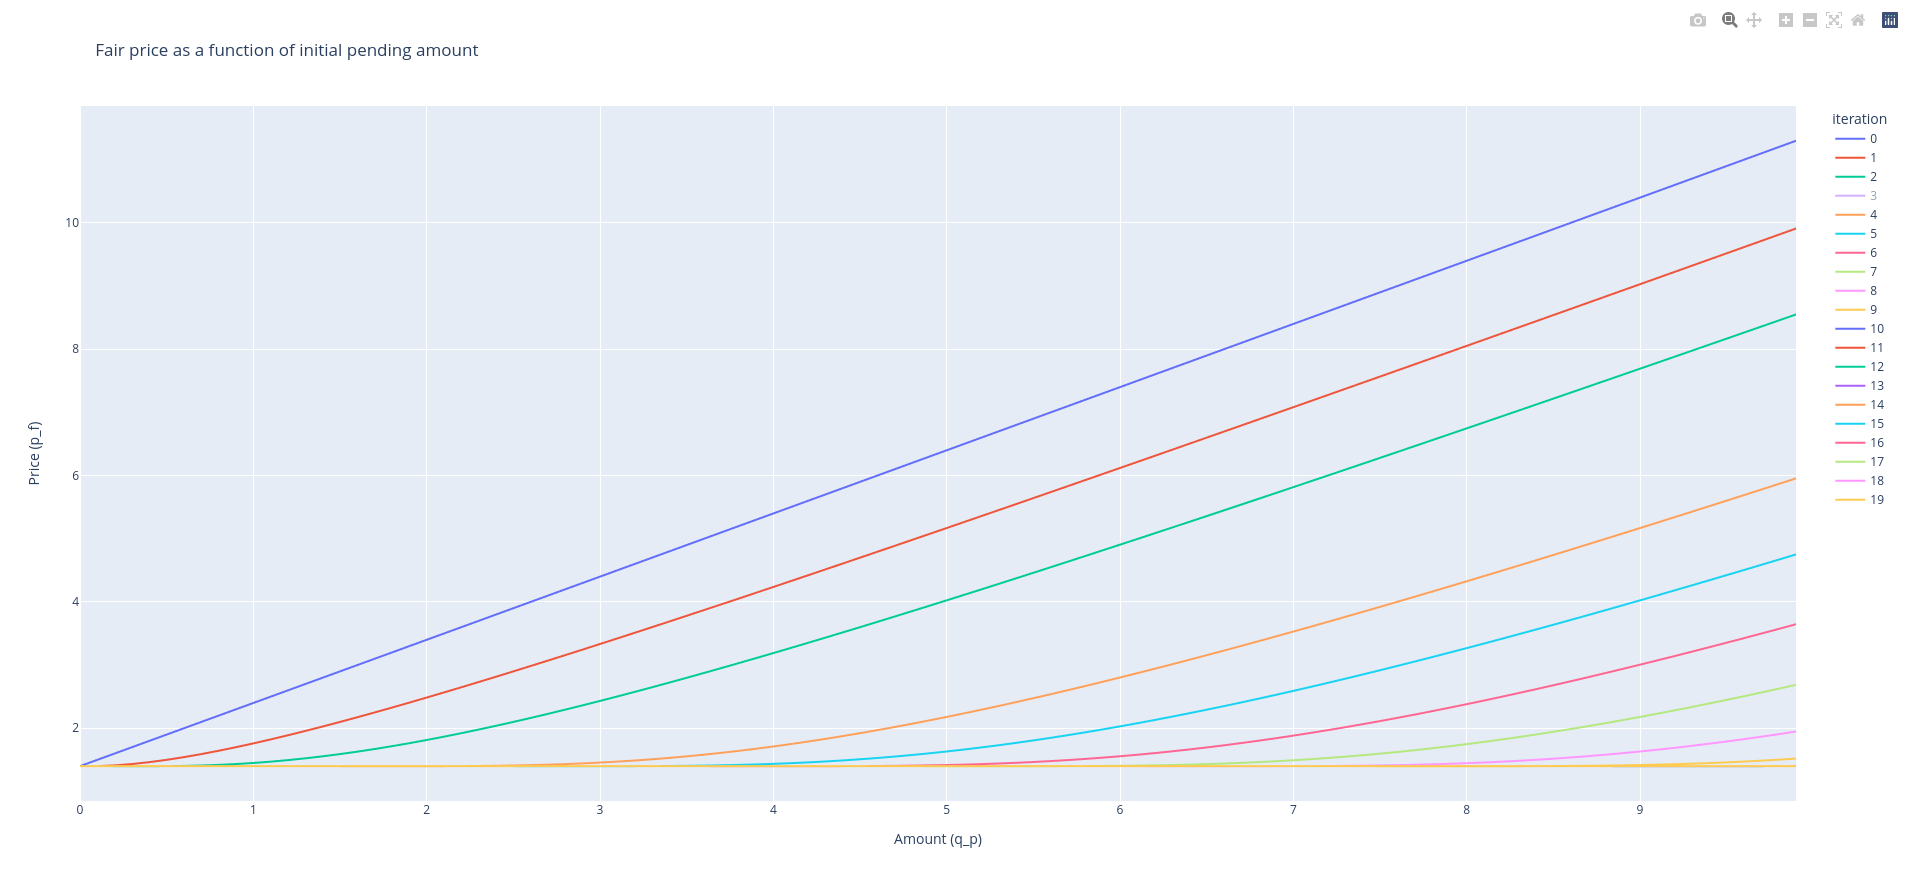
\includegraphics[width=\linewidth]{./ChickenBonds_Whitepaper_recursive_price_1.png}

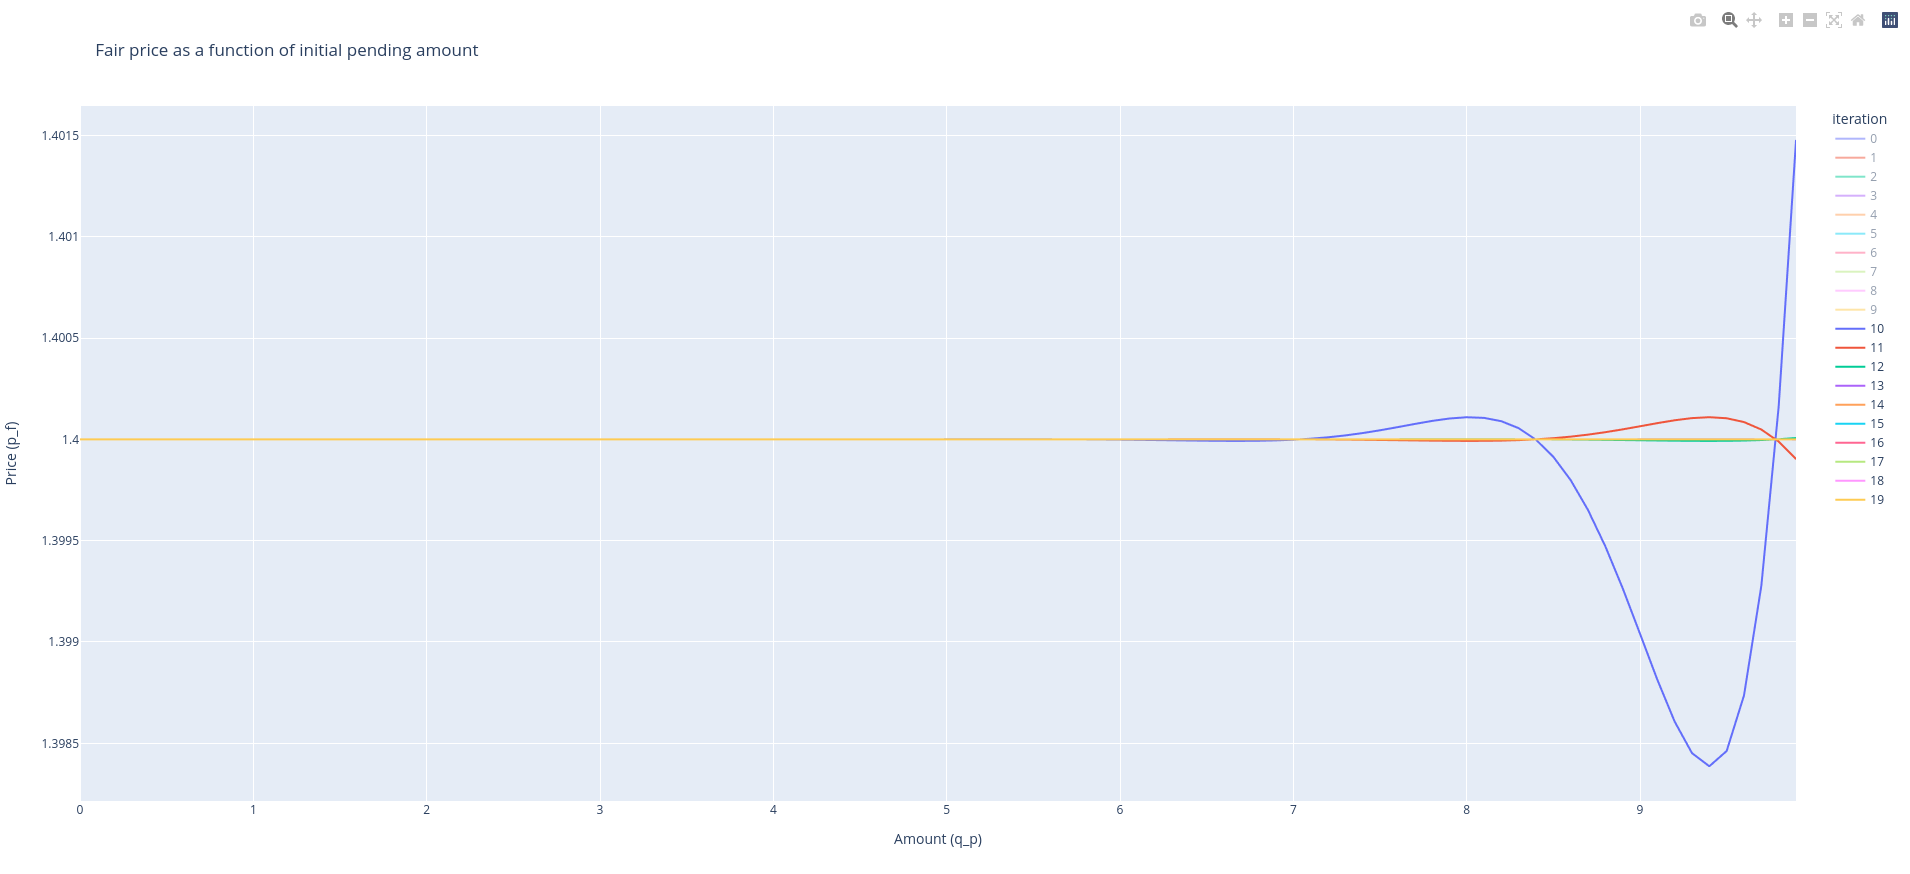
\includegraphics[width=\linewidth]{./ChickenBonds_Whitepaper_recursive_price_2.png}

\subsubsection{Yield comparison approach}
We can also consider the evolution of the fair price of bTKN over a given time period and compare it with an expected yield. In the following, we outline two different approaches.

\paragraph{Equating ROI of bonding TKN and holding bTKN}
We suppose that users would bond TKN rather than stake bTKN if the expected ROI from bonding is higher than of (buying and) holding bTKN, and vice versa. As long as holding bTKN is more attractive than bonding TKN, we can expect buying pressure on bTKN. Conversely, there should be selling pressure on bTKN if bonding is seen as more profitable since people would likely trade their bTKN for TKN. 

As a consequence, there must be an equilibrium price at which holding bTKN and bonding TKN result in the same ROI for both activities. Due to the yield amplification, it's safe to assume that in the long run, holding bTKN is at least as profitable as staking TKN. We further assume that the price of TKN is already “arbitraged” and adapted to the natural rate $r_m$, which thus carries over to the price of bTKN. Therefore, the equilibrium price for bonding vs. holding should also be meaningful as a metric for the fair price.

We now consider one optimal rebonding period $T_{opt}$, making the simplifying assumption that the price premium $\lambda$ stays constant during that time frame. Thus, the fair price $p_f$ changes from $t$ to $T_{opt}$ at the same rate as the redemption price $p_r$, yielding the ROI of holding bTKN:

\begin{equation}
  \label{eq:ROI-eq}
  H_{ROI} = \frac{p_f(t + T_{opt}) - p_f(t)}{p_f(t)} = \frac{p_r(t + T_{opt}) - p_r(t)}{p_r(t)}
\end{equation}

The resulting redemption price at time $t + T_{opt}$ can be expressed by
\begin{equation}
  \label{eq:redemption-price}
    p_r(t + T_{opt}) = \frac{q_a + \frac{T_{opt}}{365} (r_p q_p + r_a q_a + r_d q_d)}{S}
\end{equation}

yielding:
\begin{equation}
  \label{eq:ROI-eq2}
  \begin{split}
    H_{ROI} & = \frac{\frac{q_a + \frac{T_{opt}}{365} (r_p q_p + r_a q_a + r_d q_d)}{S} - p_r(t)}{p_r(t)} \\
    & = \frac{q_a}{S \cdot p_r(t)} + \frac{\frac{T_{opt}}{365} (r_p q_p + r_a q_a + r_d q_d)}{S\cdot p_r(t)} - \frac{p_r(t)}{p_r(t)} \\
    & = 1 + \frac{T_{opt}}{365} \frac{r_p q_p + r_a q_a + r_d q_d}{q_a} - 1 \\
    & = \frac{T_{opt}}{365} \frac{r_p q_p + r_a q_a + r_d q_d}{q_a}
  \end{split}
\end{equation}

On the other hand, we can express the ROI of bonding TKN for the same period as:

\begin{equation}
  \label{eq:ROI-bonding}
  \begin{split}
    B_{ROI} & = \frac{p_f(t+T_{opt})}{p_r(t+T_{opt})}\frac{T_{opt}}{T_{opt}+\alpha} - 1 \\
    & = \frac{p_f(t)(1 + \frac{T_{opt}}{365} (r_p q_p + r_a q_a + r_d q_d))} {p_r(t)(1 + \frac{T_{opt}}{365} (r_p q_p + r_a q_a + r_d q_d))}    \frac{T_{opt}}{T_{opt}+\alpha} - 1 \\ 
    & = \frac{p_f(t)}{p_r(t)}\frac{T_{opt}}{T_{opt}+\alpha} - 1
  \end{split}
\end{equation}

Setting the two ROIs equal, and using equation \ref{eq:optimal_chicken_in_2} as an approximation of $T_{opt}$, we can solve the following equation for $p_f$:
\begin{equation}
  \label{eq:ROI-bonding-holding}
  B_{ROI} = H_{ROI}
\end{equation}

and get:
\begin{equation}
  \label{eq:ROI-bonding-holding-2}
  p_f = p_r\left(1 + \frac{T_{opt}}{365} \frac{r_p q_p + r_a q_a + r_d q_d}{q_a}\right) \frac{T_{opt}+\alpha}{T_{opt}}
\end{equation}

\paragraph{Equating ROI of staking TKN and holding bTKN}
Assuming rational markets and no additional risks for holding bTKN compared to holding (and staking) TKN, we suppose that the market price of bTKN would grow at the same rate as the value of staked TKN. The rationale being that if the market expects bTKN to grow faster in the future, it should pay a higher price for bTKN now, meaning that the initial price premium should reflect the future growth potential and cancel out any oversized yield from the start. (Or is economically possible under perfectly rational conditions that a portfolio A has a higher yield than a portfolio B with the same risk profile?)

If we know what yield to expect, we could formulate a differential equation to derive a formula for $p_f$ or at least a parameter $\gamma$ for the impact of the pending bucket in the naive formula:

\begin{equation}
  \label{eq:naive-beta}
   p_f = \frac{q_a + \gamma q_p + q_d \cdot \frac{r_d}{r_a} \cdot d_f}{S}
\end{equation}

We could then state the following equation:

\begin{equation}
  \label{eq:yield-eq}
  \frac{p_f(t + 365) - p_f(t)}{p_f(t)} = r_s = r_m 
\end{equation}

Given that people would rebond during the course of the year, it’s simpler to consider a time period that corresponds to an optimal rebonding period for the current premium, which we suppose to be constant as long as no rebonding happens (all else being equal). This means, we assume away any new bonds and chicken-outs, and only consider the group of existing bonders which all rebond perfectly.

This allows us to reformulate the equation, which could be solved for $\gamma$:

\begin{equation}
  \label{eq:yield-eq}
  \frac{p_f(t + T_{opt}) - p_f(t)}{p_f(t)} = \frac{T_{opt}}{365} r_m
\end{equation}

\subsubsection{Conservative approach}
This approach is probably not the most accurate or realistic, but at least it can serve as a lower bound for the fair price.

Let’s imagine a user who wants to buy bTKN to sell it after some time $T$, and, being conservative, they don’t want to rely on other users making the same valuations, but to make sure that even reedeming their bTKN they would at least make the gains corresponding to the natural rate.

In the following chart, red line would correspond to the natural rate, green one to the redemption price and purple one to the (conservative) fair price.

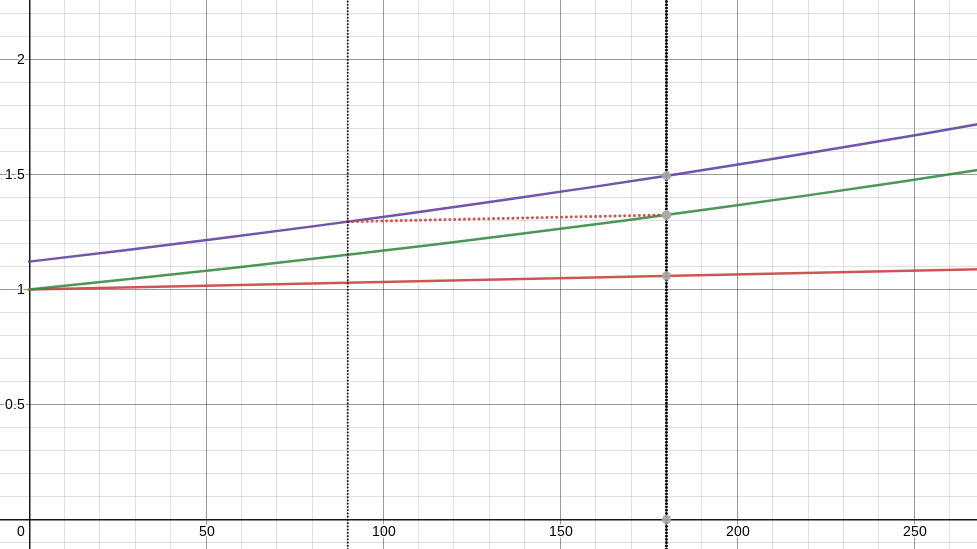
\includegraphics[width=\linewidth]{./ChickenBonds_Whitepaper_conservative_price.png}

The formula therefore for the conservative fair price would be:

\begin{equation}
  \label{eq:conservative-1}
p_f(t) = p_r(t + T) - (n(t+T) - n(t))
\end{equation}

Where $n(t)$ would represent the natural rate.

Assuming time $t$ to be denominated in days, the daily natural rate $r_m$ is expected to be low, so for values of $t$ in the order of magnitude of a year we can use the following approximation:

\begin{equation}
  \label{eq:conservative_natural_approximation}
n(t) = (1 + r_m)^t = 1 + r_m \cdot t
\end{equation}

We need to find then a formula for $p_r$ and we are all set.

\paragraph{With rebonding}
With rebonding this is quite hard, as we need optimal rebonding time $T_{opt}$, which in turn uses fair price (see \ref{sec:T_OP}).

If we assume that redemption price has an exponential behavior, due to the compounding effect of rebonding, of the form $p_r = a^t$ \footnote{This is probably wrong, as we will see in the no rebonding case!}, then fair price would be (using approximation in \ref{eq:conservative_natural_approximation}):

\begin{equation}
  \label{eq:conservative-2}
p_f(t) = a^{t+T} - r_m T
\end{equation}

Let’s try to find $a$.

For $t=0$, ${q_a}_0 = S_0$ and $p_r(0) = 1$. See \ref{sec:bootstrapping}.

Optimal rebonding time (using \ref{eq:optimal_chicken_in_1} and assuming $\alpha = 1$ to simplify):

\begin{equation}
  \label{eq:conservative_T_OP}
T_{opt} = \frac{1+ \sqrt{a^T - r_mT}}{a^T - r_mT - 1}
\end{equation}

The corresponding issuance proportion:

\begin{equation}
  \label{eq:conservative_issuance_proportion}
  \begin{split}
  \frac{T_{opt}}{T_{opt} + 1} & = \frac{\frac{1+ \sqrt{a^T - r_mT}}{a^T - r_mT - 1}}{\frac{1+ \sqrt{a^T - r_mT}}{a^T - r_mT - 1} + 1} \\
  & = \frac{1+ \sqrt{a^T - r_mT}}{1+ \sqrt{a^T - r_mT} + a^T - r_mT - 1} \\
  & = \frac{1+ \sqrt{a^T - r_mT}}{a^T - r_mT + \sqrt{a^T - r_mT}} \\
  & = \frac{(1+ \sqrt{a^T - r_mT})(a^T - r_mT - \sqrt{a^T - r_mT})}{(a^T - r_mT)^2 + a^T - r_mT} \\
  & = \frac{a^T - r_mT - \sqrt{a^T - r_mT} + (a^T - r_mT)\sqrt{a^T - r_mT} - (a^T - r_mT)}{(a^T - r_mT)(a^T - r_mT - 1)} \\
  & = \frac{- \sqrt{a^T - r_mT} + (a^T - r_mT)\sqrt{a^T - r_mT}}{(a^T - r_mT)(a^T - r_mT - 1)} \\
  & = \frac{(a^T - r_mT - 1)\sqrt{a^T - r_mT}}{(a^T - r_mT)(a^T - r_mT - 1)} \\
  & = \frac{\sqrt{a^T - r_mT}}{a^T - r_mT} \\
  & = \frac{1}{\sqrt{a^T - r_mT}}
  \end{split}
\end{equation}

Now moving forward to $t_1 = T_{opt}$:

\[
{q_p}_1 = {q_p}_0 \frac{a^T -r_mT}{\sqrt{a^T -r_mT}} = {q_p}_0 \sqrt{a^T - r_mT}
\]

\[
{q_a}_1 = {q_a}_0 + [({q_a}_0 + {q_p}_0)r_s + {q_d}_0 r_d] T_{opt} + {q_p}_0 \frac{1}{\sqrt{a^T - r_mT}}
\]

\[
S_1 = S_0 + \frac{{q_p}_0}{\sqrt{a^T - r_mT}} = {q_a}_0 + \frac{{q_p}_0}{\sqrt{a^T - r_mT}}
\]

So finally:

\begin{equation}
  \label{eq:conservative_p_r_1}
  \begin{split}
    {p_r}_1 & = \frac{{q_a}_1}{S_1} \\
    & = \frac{{q_a}_0 + [({q_a}_0 + {q_p}_0)r_s + {q_d}_0 r_d] T_{opt} + {q_p}_0 \frac{1}{\sqrt{a^T - r_mT}}}{{q_a}_0 + \frac{{q_p}_0}{\sqrt{a^T - r_mT}}} \\
    & = 1 + \frac{({q_a}_0 + {q_p}_0)r_s + {q_d}_0 r_d + {q_p}_0}{{q_a}_0 + \frac{{q_p}_0}{\sqrt{a^T - r_mT}}} \frac{1+ \sqrt{a^T - r_mT}}{a^T - r_mT - 1} \\
  \end{split}
\end{equation}

If we now equate this to $p_r(T_{opt})$ we get:
\begin{equation}
  \label{}
1 + \frac{({q_a}_0 + {q_p}_0)r_s + {q_d}_0 r_d + {q_p}_0}{{q_a}_0 + \frac{{q_p}_0}{\sqrt{a^T - r_mT}}} \frac{1+ \sqrt{a^T - r_mT}}{a^T - r_mT - 1} = a ^{\frac{1+ \sqrt{a^T - r_mT}}{a^T - r_mT - 1}}
\end{equation}

which seems quite hard to solve for $a$.

\paragraph{Without rebonding}

Although this approach without rebonding quite misses the point, as redemption price would be too close to natural rate, we can still try:

Now we only account for the yield generated, which doesn’t increase the bTKN total supply:

\[
S_t = S_1 = S_0 = {q_a}_0
\]

We try to compute acquired bucket for several time intervals, let’s say daily:

\[
{q_a}_1 = {q_a}_0 + [({q_a}_0 + {q_p}_0) r_s + {q_d}_0 r_d] = {q_a}_0 + {q_a}_0 r_s + {q_p}_0 r_s + {q_d}_0 r_d
\]

\[
{q_a}_t = {q_a}_0(1+r_s)^t + ({q_p}_0 r_s + {q_d}_0 r_d) \left(r_s^t + \sum_{j=1}^{t-1} \binom{t}{j} a^j \right)
\]

So for time $t$ the redemption price would be:

\[
p_r(t) = \frac{{q_a}_t}{S_1} = \frac{{q_a}_0(1+r_s)^t + ({q_p}_0 r_s + {q_d}_0 r_d) \left(r_s^t + \sum_{j=1}^{t-1} \binom{t}{j} a^j \right)}{{q_a}_0}
\]

\begin{equation}
  \label{eq:conservative_p_r_base_2_a}
p_r(t) = (1+r_s)^t + \frac{{q_p}_0 r_s + {q_d}_0 r_d}{{q_a}_0} \left(r_s^{t-1} + \sum_{j=1}^{t-1} \binom{t}{j} r_s^{t-1-j} \right)
\end{equation}

We can approximate it to:

\begin{equation}
  \label{eq:conservative_p_r_base_2_b}
p_r(t) = (1+r_s)^t + \frac{{q_p}_0 r_s + {q_d}_0 r_d}{{q_a}_0} t
\end{equation}

In particular this shows that the assumption that redemption price follows a pure exponential $a^t$ is not correct.

\subsection{Effect of chicken ins and rebonding on the fair price}
TODO: update once we have a formula for the fair price

\subsection{Self-reinforcing price impact}
It follows from equations \ref{eq:opt-rebonding} that a higher premium $\lambda$ leads to a shorter rebonding period $t$ (the same is true for \ref{eq:optimal_chicken_in_2}, and for break even time in \ref{eq:break_even_2}). As a consequence, we can expect bonders to chicken in earlier, resulting in a higher fraction of the bond $b_p$ that transitions into the Permanent Bucket, which has a reinforcing effect on the premium and is favorable for the fair price of bTKN (see TODO).

Thus, if the market price of bTKN increases while everything else stays equal, the chances are higher that the price will continue to rise in the future thanks to earlier chicken ins. While this effect may be not always be immediate, a large bTKN price hike could effectively push bonders beyond their optimal rebonding times.
Assuming perfectly rational behavior, this would result in immediate chicken ins (and rebonding).

TODO: check and update once we have a formula for the fair price

\subsection{Self-stabilizing effect of redemptions and its help to regain traction}
  \label{sec:self-stabilizing}
As redemptions reduce the Acquired Bucket and the bTKN supply in the same proportion, they indirectly increase the impact of the Permanent and the Pending Bucket on bTKN through a higher yield amplification. While the redemption price doesn't change when somebody redeems bTKN for TKN, the fair price and thus the expected premium grow as a result. 

We can therefore expect a self-stabilizing effect of redemptions: for any given $q_p \geq 0$ and $q_d > 0$ there should be an equilibrium state with $q_a > 0$ where $p_r = p_f$, making further redemptions and a complete drainage of the Acquired Bucket unlikely. Given this de facto lower bound on $q_a$, a portion of the Acquired Bucket will behave as if it was permanent.

Furthermore, natural fluctuations of the market price $p_m$ compared to $p_f$ could help the system regain traction should it ever reach a state where $p_f = p_r$: if the market temporarily prices the bTKN below its fair price ($p_m < p_f$), redemptions will kick in and raise $p_f$, increasing the odds that the market will return to $p_m > p_r$ and make bonding attractive again. This dynamic should apply even if $q_p = 0$, i.e. when bonding activity has come to a complete halt.

\section{Protocol enhancements}
\subsection{Bootstrapping}
  \label{sec:bootstrapping}
Right after launch, the initial bTKN supply will be 0 as the token is only minted upon chicken in events. Similarly, the Acquired Bucket is empty until the first bond holder chickens in. As a result, the redemption price $p_r$ (backing ratio) is undefined and cannot be used for calculating the accrued amount $s(t)$ during this bootstrapping period.

Meanwhile, the protocol already starts earning yield on the Pending Bucket before anybody chickens in. For fairness reasons, we want to ensure that this initial yield isn't simply earned by the bond holder who chickens in first.

To tackle this bootstrapping problem, we define the initial redemption price at the time of the first chicken in to be $p_r = 1$. The protocol thus needs to mint the same amount of bTKN as the amount of TKN acquired by the protocol up to that time. The accumulated yield of the Pending Bucket, which would normally belong to the Acquired Bucket, can be used to bootstrap a bTKN/TKN DEX pair, as the protocol can mint the bTKN to fill the other side of the AMM.

To make sure that the initial AMM price reflects the initial redemption price of 1, the system needs to deposit the same nominal amount of bTKN and TKN to the respective pool. So, it can use $50\%$ of the accumulated yield (in TKN) to bootstrap the AMM, while moving the other half into the Acquired Bucket. The part of the yield used to bootstrap the AMM is technically also considered as being "acquired" and is thus reflected in $q_a$, such that $q_a = S$ holds upon the very first chicken in, ensuring $p_r = 1$.

\subsection{Two-bucket version}
\label{sec:two-bucket}
A Permanent Bucket may not be suitable for all use cases and protocol tokens. For example, if TKN is a token that is minted through loans, keeping a portion of it inside the Permanent Bucket forever would essentially reduce the circulating supply, which could impact the ability of borrowers to repay their debts. On the other hand, such tokens have usually no fixed or capped supply, but can be minted as needed, meaning that technically there's an unbounded amount of TKN that could be bonded over time.

This makes bonding more sustainable in the long run even without a Permanent Bucket.


\subsection{Auto-adjusting the steepness $\alpha$ of the accrual curve}
  \label{sec:adjustment}
TODO

\subsection{Redemption fees}
  \label{sec:redemption-fee}
To throttle the outflow of TKN from the Acquired Bucket, the system may charge a fee on redemptions, called the \textit{redemption fee}. The redeemer of $n$ bTKN would then get slightly less TKN than their pro rata share, i.e. $x < n \cdot p_r$. The difference $(n \cdot p_r - x)$ could be either kept in the Acquired Bucket or moved to the Permanent Bucket. 

In both cases, the captured fee increases the fair price by the same amount, in addition to the positive effect of the redemption as such on $p_f$ (see \ref{sec:self-stabilizing}). However, in the first case, the redemption price $p_r$ also increases, decreasing the premium compared to a baseline without any redemption fee, while in the second case the premium grows more than in the baseline. TODO: give some mathematical intuition on this.

\subsubsection{Determining the fee}
TODO

\subsection{Payout tax as an incentive for the bTKN/TKN DEX pair}
  \label{sec:payout-tax}
TODO

\end{document}
